\chapter{Задание}

\textbf{Цель работы}: построение гистограммы и эмпирической функции распределения.

\begin{enumerate}
	\item Для выборки объема $n$ из генеральной совокупности $X$ реализовать в виде программы на ЭВМ
		\begin{enumerate}
			\item вычисление максимального значения $M_{\max}$ и минимального значения $M_{\min}$;
			\item размаха $R$ выборки;
			\item вычисление оценок $\hat\mu$ и $S^2$ математического ожидания $MX$ и дисперсии $DX$;
			\item группировку значений выборки в $m = [\log_2 n] + 2$ интервала;
			\item построение на одной координатной плоскости гистограммы и графика функции плотности распределения вероятностей нормальной случайной величины с математическим
ожиданием $\hat\mu$ и дисперсией $S^2$;
			\item построение на другой координатной плоскости графика эмпирической функции распределения и функции распределения нормальной случайной величины с математическим
ожиданием $\hat\mu$ и дисперсией $S^2$.
		\end{enumerate}
	\item Провести вычисления и построить графики для выборки из индивидуального варианта.
\end{enumerate}

\chapter{Теоретическая часть}

Пусть дана выборка $$\vec x=(x_1, ..., x_n)$$ объема $n$ из генеральной совокупности $X$.

\section{Формулы для вычисления величин}

\textbf{Максимальное и минимальное значения выборки}
\begin{equation}
    \begin{aligned}
        M_{\max} = \max\{x_1, .., x_n\}\\
        M_{\min} = \min\{x_1, .., x_n\}
    \end{aligned}
\end{equation}

\textbf{Размах выборки}
\begin{equation}
    R = M_{\max} - M_{\min}
\end{equation}

\textbf{Оценки математического ожидания и дисперсии}

Выборочное среднее:

\begin{equation}
    \begin{aligned}
    \hat \mu(\vec x) = \frac{1}{n} \sum_{i=1}^n x_i
    \end{aligned}
\end{equation}

Исправленная выборочная дисперсия:

\begin{equation}
    \begin{aligned}
    S^2(\vec x) = \frac{1}{n-1} \sum_{i=1}^n (x_i - \overline x)^2,
    \end{aligned}
\end{equation}

где $ \overline{x} = \hat \mu $

\section{Определение эмпирической плотности и гистограммы}

Пусть $\vec x$ --- выборка из генеральной совокупности $X$. Если объем этой выборки $n$ достаточно велик, то значения $x_i$ группируют в интервальный статистический ряд. Для этого отрезок $J = [x_{(1)}, x_{(n)}]$ разбивают на $m$ равновеликих промежутков. Ширина каждого из них:

\begin{equation}
    \Delta = \frac{|J|}{m} = \frac{x_{(n)} - x_{(1)}}{m}
\end{equation}

Полагают

\begin{equation}
    J_i = [x_{(1)} + (i - 1) \cdot \Delta, x_{(1)} + i \cdot \Delta), i = \overline{1; m - 1}
\end{equation}

\begin{equation}
    J_{m} = [x_{(1)} + (m - 1) \cdot \Delta, x_{(n)}]
\end{equation}

\textbf{Интервальным статистическим рядом}, отвечающим выборке $\vec x$, называется таблица вида

\begin{table}[htb]
    \centering
    \begin{tabular}{|c|c|c|c|c|}
        \hline
        $J_1$ & $J_2$ & ... & $J_m$ \\
        \hline
        $n_1$ & $n_2$ & ... & $n_m$ \\
        \hline
    \end{tabular}
\end{table}

где $n_i$ --- число элементов выборки $\vec x$, попавших в промежуток $J_i, i = \overline{1; m}$.

Для выбора $m$ используют формулу: 
\begin{equation}
    m = [\log_2n] + 2,
\end{equation}
где $n$ --- размер выборки.

Пусть для данной выборки $\vec x$ построен интервальный статистический ряд $(J_i, n_i), i = \overline{1; m}$.

\textbf{Эмпирической плотностью} распределения (соответствующей выборке $\vec x$) называется функция:
\begin{equation}
    f_n(x) =
    \begin{cases}
        \frac{n_i}{n \Delta}, \text{если } x \in J_i,\\
        0, \text{иначе.} \\
    \end{cases}
\end{equation}

График эмпирической функции плотности называется \textbf{гистограммой}.

\section{Определение эмпирической функции распределения}

Пусть $\vec x = (x_1, ..., x_n)$ --- выборка из генеральной совокупности $X$.\newlineОбозначим $n(t, \vec x)$ --- число компонент вектора $\vec x$, которые меньше, чем $t$.

\textbf{Эмпирической функцией распределения}, построенной по выборке $\vec x$, называют функцию

\begin{equation}
    F_n: \mathbb{R} \to \mathbb{R}, 
\end{equation}

определенную правилом

\begin{equation}
    F_n(t) = \frac{n(t, \vec x)}{n}
\end{equation}

\chapter{Практическая часть}

\section{Текст программы}

\begin{lstlisting}[style={Matlab}]
function lab_01
    X = [14.90,14.40,13.56,15.55,13.97,16.33,14.37,13.46,15.51,14.69,...
         13.41,14.24,15.65,14.54,13.55,13.15,14.32,15.04,13.27,14.60,...
         13.83,13.93,14.11,14.15,15.48,15.96,14.46,13.87,13.67,15.30,...
         13.95,16.08,18.25,14.93,15.37,14.38,15.56,13.92,14.23,12.80,...
         13.16,13.89,14.24,13.90,12.82,13.20,13.89,13.50,13.44,16.13,...
         14.68,15.27,13.35,13.62,16.16,16.46,13.83,14.13,15.68,15.22,...
         12.59,12.94,13.09,16.54,14.61,14.63,14.17,13.34,16.74,16.30,...
         13.74,15.02,14.96,15.87,16.03,12.87,14.32,14.48,14.57,14.43,...
         12.61,14.52,15.29,12.07,14.58,11.74,14.97,14.31,12.94,12.82,...
         14.13,14.48,12.25,14.39,15.08,12.87,14.25,15.12,15.35,12.27,...
         14.43,13.85,13.16,16.77,14.47,14.89,14.95,14.55,12.80,15.26,...
         13.32,14.92,13.44,13.48,12.81,15.01,13.19,14.68,14.44,14.89];

    X = sort(X);
    n = length(X);

    M_max = max(X);
    M_min = min(X);
    fprintf("\nМаксимальное значение = %.4f\n", M_max);
    fprintf("Минимальное значение = %.4f\n", M_min);

    R = M_max - M_min;
    fprintf("\nРазмах выборки = %.4f\n", R);

    mu = sum(X) / n;
    S2 = sum((X-mu).^2) / (n - 1);
    fprintf("\nОценка математического ожидания = %.4f\n", mu);
    fprintf("Оценка дисперсии = %.4f\n", S2);

    m = floor(log2(n)) + 2;
    fprintf("\nЧисло интервалов = %d\n\n", m);

    d = (X(n) - X(1)) / m;

    J = [];

    for i = 1 : m
      J(i, 1) = X(1) + (i - 1) * d;
      J(i, 2) = X(1) + i * d;
    end
 
    N = zeros(m);
    
    for i = 1 : n
      for j = 1 : m
        if X(i) >= J(j, 1) && X(i) < J(j, 2)
          N(j)++;
        end
      end
    end
    
    N(m)++;
    
    for i = 1 : m - 1
      fprintf("[%.4f,%.4f) - %d\n", J(i, 1), J(i, 2), N(i));
    end
    
    fprintf("[%.4f,%.4f] - %d\n", J(m, 1), J(m, 2), N(m));

    f = [];
    
    for i = 1 : m
      f(i, 1) = (J(i, 1) + J(i, 2)) / 2;
      f(i, 2) = N(i) / (n * d);
    end
    
    args = X(1):1e-4:X(n);
    sigma = sqrt(S2);
    f_normal = normpdf(args, mu, sigma);

    bar(f(:,1), f(:,2), 1, "b");
    hold on;
    plot(args, f_normal, 'g', 'LineWidth', 2);
    grid;

    F = [];
    
    F(1, 2) = 0;
    F(1, 1) = X(1) - 1;
    
    for i = 2 : (n + 1)
      cnt = 0;
      for j = 1 : n
        if X(j) <= X(i - 1)
          cnt++;
        end
      end
      
      F(i, 1) = X(i - 1);
      F(i, 2) = cnt / n;
    end

    F(n + 2, 2) = 1;
    F(n + 2, 1) = X(n) + 1;

    F_normal = normcdf(args, mu, sigma);

    figure;
    stairs(F(:,1), F(:,2), "b");
    hold on;
    plot(args, F_normal, "r", 'LineWidth', 2);
    grid;
endfunction
\end{lstlisting}

\section{Результаты расчетов для выборки из индивидуального варианта}

\begin{lstlisting}[style={Matlab}]
Максимальное значение = 18.2500
Минимальное значение = 11.7400

Размах выборки = 6.5100

Оценка математического ожидания = 14.3492
Оценка дисперсии = 1.2776

Число интервалов = 8

[11.7400,12.5538) - 4
[12.5538,13.3675) - 21
[13.3675,14.1813) - 27
[14.1813,14.9950) - 37
[14.9950,15.8087) - 18
[15.8087,16.6225) - 10
[16.6225,17.4363) - 2
[17.4363,18.2500] - 1
\end{lstlisting}

\begin{figure}[H]
	\begin{center}
		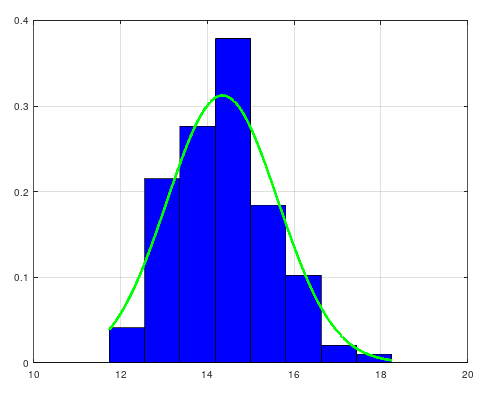
\includegraphics[scale=0.8]{img/bar.png}
	\end{center}
	\captionsetup{justification=centering}
	\caption{Гистограмма и график функции плотности распределения нормальной случайной величины с математическим ожиданием $\hat\mu$ и дисперсией $S^2$}
	\label{img:bar}
\end{figure}

\begin{figure}[H]
	\begin{center}
		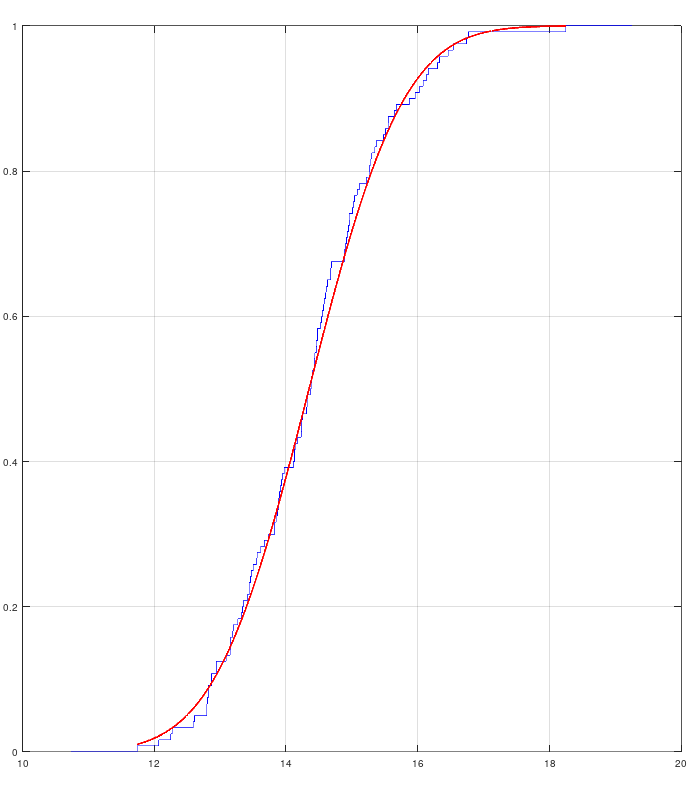
\includegraphics[scale=0.6]{img/graph.png}
	\end{center}
	\captionsetup{justification=centering}
	\caption{График эмпирической функции распределения и функции распределения нормальной случайной величины с математическим ожиданием $\hat\mu$ и дисперсией $S^2$}
	\label{img:graph}
\end{figure}